\documentclass[hyperref={pdfpagelabels=false}]{beamer}

% Pacotes ----------------------------------------------------------------------
\usepackage[utf8]{inputenc}
\usepackage[T1]{fontenc}
\usepackage[brazil]{babel}
\usepackage{amsmath}
\usepackage{listings}

% Configurações Especializadas -------------------------------------------------
\setbeamertemplate{navigation symbols}{}
\let\Tiny=\tiny

% Dados Pessoais ---------------------------------------------------------------
\title[\LaTeX{}]{\LaTeX{} Workshop}
\subtitle{Mini Curso de Introdução ao \LaTeX{}}
\author[CAMARGO]{Wanderson Henrique Camargo Rosa}
\institute[UNISINOS]{Universidade do Vale do Rio dos Sinos --- UNISINOS}
\date{\today{}}
\keywords{latex sbc}

% Agenda -----------------------------------------------------------------------
\AtBeginSubsection[]
{
\begin{frame}{Agenda}
    \tableofcontents[currentsection,currentsubsection]
\end{frame}
}

% Início do Documento ----------------------------------------------------------
\begin{document}

% Página Inicial ---------------------------------------------------------------
\begin{frame}
    \maketitle{}
    \begin{center}
        
\includegraphics[width=20mm]{src/CC-BY-NC-SA-icon-88x31.png}
    \end{center}
\end{frame}

% Agenda -----------------------------------------------------------------------
\begin{frame}{Agenda}
    \tableofcontents{}
\end{frame}

% Apresentação -----------------------------------------------------------------
\section{Apresentação}
\label{sec:apresentacao}

\subsection{Informações}

\begin{frame}{Objetivo}
    Criar um artigo que esteja padronizado conforme as normas da Sociedade
    Brasileira de Computação (SBC), disponibilizadas em pacote específico pela
    instituição, utilizando \LaTeXe{} e ferramentas de código aberto.
\end{frame}

\begin{frame}{Aptidões Adquiridas}
    O aluno estará apto a criar um artigo simples, segundo as normas da SBC
    fornecidas, bem como poderá pesquisar conteúdos sobre \LaTeX{} nas
    bibliografias exibidas, filtrando informações relevantes durante a busca.
\end{frame}

\begin{frame}{Problemas Encontrados}
    A acentuação em exemplos está incorreta pois o pacote responsável pela
    demonstração de códigos no formato \TeX{} não foi devidamente configurado.
\end{frame}

% Introdução -------------------------------------------------------------------
\section{Introdução}
\label{sec:introducao}

\subsection{Histórico}

\begin{frame}{Definição}
    \LaTeX{} é um sistema de composição de textos\cite{oetiker2008}, adequado
    para produção de documentos matemáticos de alta qualidade tipográfica. É uma
    versão especial do \TeX{} que entende comandos próprios\cite{lamport1994} e
    trabalha buscando dividir as funções de formatação do documento e ordem
    lógica do texto.
\end{frame}

\begin{frame}{Donald Knuth e \TeX{}}
    \begin{itemize}
        \item Grande Contribuidor para a Computação
        \item Programação Literária
        \item Insatisfeito com a Qualidade dos Documentos
    \end{itemize}
    \pause{}
    \begin{figure}
        \centering{}
        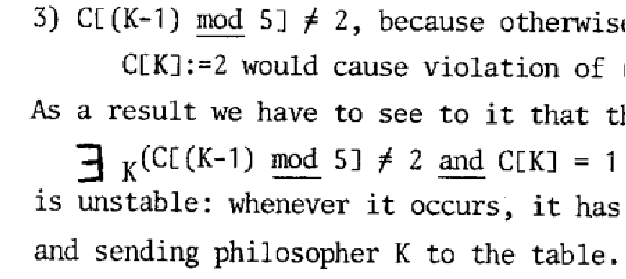
\includegraphics[scale=0.5]{src/dijkstra.png}
        \caption{Dijkstra e o Jantar dos Filósofos}
        \label{fig:dijkstra}
    \end{figure}
\end{frame}

\begin{frame}[fragile]{Leslie Lamport e \LaTeX{}}
    \begin{itemize}
        \item Cientista da Computação
        \item Teoria de Sistemas Distribuídos
        \item Dificuldade de Utilização do \TeX{}
    \end{itemize}
    \pause{}
    \begin{block}{Bhaskara}
        \begin{equation*}
            \frac{-b\pm\sqrt{b^2-4ac}}{2a}
        \end{equation*}
        \centering{}
        \verb,\frac{-b\pm\sqrt{b^2-4ac}}{2a},
    \end{block}
\end{frame}

\subsection{Informações}

\begin{frame}{\LaTeX{}}
    \begin{itemize}
        \item Vantagens\cite{oetiker2008}
        \begin{itemize}
            \item Padrões Profissionais;
            \item Suporte Nativo para Matemática;
            \item Divisão Lógica do Documento; e
            \item Rodapé, Referências Cruzadas e Índice Automáticos.
        \end{itemize}
        \item Desvantagens
        \begin{itemize}
            \item Dificuldade para Modificar Formatos;
            \item Escrita de Documentos sem Ordem Lógica; e
            \item Aparência Inicial Complicada.
        \end{itemize}
    \end{itemize}
\end{frame}

\begin{frame}{Idéia Principal}
    \LaTeX{}\cite{oetiker2008} habilita o autor do documento a formatar o seu
    próprio trabalho com qualidade profissional usando formatos
    \alert{pré-definidos}.
    \pause{}
    \begin{block}{Formatos Disponíveis (Entre Muitos Outros)}
        \begin{center}
            Associação Brasileira de Normas Técnicas (ABNT)\\
            Institute of Eletrical and Eletronics Engineers (IEEE)\\
            Sociedade Brasileira de Computação(SBC)
        \end{center}
    \end{block}
\end{frame}

\begin{frame}{Informações Adicionais}
    \begin{center}
        \huge{Multiplataforma}
    \end{center}
    \begin{itemize}
        \item Arquivos Gerados
        \begin{description}
        \item[DVI] Device Independent
        \item[PS]  Postscript
        \item[PDF] Adobe Pocket Document
        \end{description}
        \pause{}
        \item Ambientes de Interface
        \begin{columns}[c]
            \begin{column}{0.5\textwidth}
                \begin{itemize}
                    \item Windows
                    \begin{itemize}
                        \item Mik\TeX{}
                        \item WinEdt
                        \item \TeX{}nicCenter
                        \item WinShell
                        \item \TeX{}maker
                        \item Emacs
                        \item \LaTeX{} Editor
                    \end{itemize}
                \end{itemize}
            \end{column}
            \begin{column}{0.5\textwidth}
                \begin{itemize}
                    \item Linux
                    \begin{itemize}
                        \item \TeX{}maker
                        \item Vim
                        \item \TeX{}Live
                        \item Kile
                        \item Gedit
                        \item Emacs
                        \item Lyx
                    \end{itemize}
                \end{itemize}
            \end{column}
        \end{columns}
    \end{itemize}
\end{frame}

% Documento --------------------------------------------------------------------
\section{Documento}
\label{sec:documento}

\subsection{Estrutura Inicial}

\begin{frame}[fragile]{Estrutura de Arquivo}
    \begin{columns}[t]
        \begin{column}{0.5\textwidth}
\begin{lstlisting}[language=TeX,basicstyle=\scriptsize]
\documentclass[opcoes]{tipo}
% Preambulo
% Comentario

\usepackage[opcoes]{pacote}

\begin{document}

    Texto e Comandos

    \begin{ambiente}[opcoes]
        Texto e Comandos
    \end{ambiente}

\end{document}
\end{lstlisting}
        \end{column}
        \begin{column}{0.5\textwidth}
\begin{lstlisting}[basicstyle=\scriptsize]
Tipo: article, book, beamer

Comentario com %

Carregamento de Pacote

Inicio do Documento

Texto

Inicio de Ambiente
    Texto
Fim de Ambiente

Fim do Documento
\end{lstlisting}
        \end{column}
    \end{columns}
\end{frame}

\begin{frame}[fragile]{Meu Documento}{Estrutura Básica}
\begin{lstlisting}[language=TeX,basicstyle=\scriptsize]
\documentclass{article}       % Documento Tipo Artigo

\usepackage[utf8]{inputenc}   % [latin1] para Windows
\usepackage[T1]{fontenc}      % Hifenizacao Correta
\usepackage[brazil]{babel} % Texto em Portugues do Brasil

\begin{document}              % Inicio Documento

    Ola, mundo!

\end{document}                % Fim Documento
\end{lstlisting}
\end{frame}

\subsection{Arquivos}

\begin{frame}{Arquivos Gerados}
    Muitos arquivos são gerados em tempo de compilação, porém os mais
    importantes nesta aplicação são:
    \begin{description}
    \item[tex] Documento Principal
    \item[bib] Bibliografia
    \item[pdf] Resultado Final
    \item[sty] Estilos e Formatação
    \end{description}
\end{frame}

\subsection{Sintaxe}

\begin{frame}{Formato de Comandos}
    \begin{itemize}
        \item Comandos \LaTeX{}
        \begin{itemize}
            \item São \emph{case sensitive} (e $\neq$ E);
            \item Iniciam por contra-barra ($\backslash$);
            \item Formados por somente letras; e
            \item Terminados por espaço, números ou não-letra.
        \end{itemize}
        \item Também são comandos
        \begin{itemize}
            \item Contra-barra seguido de não-letra.
        \end{itemize}
        \item Parâmetros estão entre chaves \{ \}
        \item Parâmetros opcionais estão entre colchetes $[$ $]$
    \end{itemize}
\end{frame}

% Personalizado ----------------------------------------------------------------
\section{Personalizando}
\label{sec:personalizando}

\subsection{Dados Pessoais}

\begin{frame}[fragile]{Meu Documento}{Dados Pessoais de Autoria}
\begin{lstlisting}[language=TeX,basicstyle=\scriptsize]
\documentclass{article}
\usepackage[utf8]{inputenc}
\usepackage[T1]{fontenc}
\usepackage[brazil]{babel}

\title{Nome do Artigo}        % Nome do Artigo
\author{Nome do Autor}        % Nome do Autor

\begin{document}
    \maketitle{}              % Construcao de Titulo
    Ola, mundo!
\end{document}
\end{lstlisting}
\end{frame}

\subsection{Pacotes}

\begin{frame}{Artigos SBC}
    A Sociedade Brasileira de Computação mantém disponível um pacote para
    formatação e documentos em \LaTeX{}, buscando padronizar seus artigos e
    livros. Acesse o site da SBC e procure o template compactado, importando o
    conteúdo para o diretório de seu documento.

    O \emph{sbc-template} possui todas as configurações para bibliografias,
    referências cruzadas e inserção de imagens com legenda, por exemplo.
\end{frame}

\begin{frame}[fragile]{Meu Documento}{Sociedade Brasileira de Computação}
\begin{lstlisting}[language=TeX,basicstyle=\scriptsize]
\documentclass{article}
\usepackage[utf8]{inputenc}
\usepackage[T1]{fontenc}
\usepackage[brazil]{babel}
\usepackage{sbc-template}

\title{Nome do Artigo}
\author{Nome do Autor}
\address{Instituicao}

\begin{document}
\maketitle{}

\begin{resumo}                % Resumo
\end{resumo}

\begin{abstract}              % Resumo em Ingles
\end{abstract}

\end{document}
\end{lstlisting}
\end{frame}

\subsection{Estruturação}

\begin{frame}[fragile]{Meu Documento}{Seções e Referências Cruzadas}
\begin{lstlisting}[language=TeX,basicstyle=\scriptsize]
...
\section{Introducao}       % 1
\label{sec:intro}
\subsection{Teoria}        % 1.1
\subsubsection{Aplicacoes} % 1.1.1
\section{Nova Teoria}      % 2
\label{sec:teoria}
\subsection{Aplicacoes}    % 2.1
...
Conforme foi dialogado na Secao \ref{sec:intro}, temos
que a nova teoria aplicada na Secao \ref{sec:teoria}
torna-se util quando...
...
\end{lstlisting}
\end{frame}

\begin{frame}[fragile]{Meu Documento}{Notas de Rodapé}
\begin{lstlisting}[language=TeX,basicstyle=\scriptsize]
...
Atraves deste principio, a aplicacao da programacao
dinamica \footnote{Estilo de algoritmos que buscam salvar
resultados ja computados} na programacao do trabalho
otimizou cerca de 95% do tempo de execucao.
...
\end{lstlisting}
\end{frame}

\begin{frame}[fragile]{Meu Documento}{Listas Numeradas e Não Numeradas}
\begin{lstlisting}[language=TeX,basicstyle=\scriptsize]
...
\begin{enumerate}
    \item Estudar o Problema;
    \item Procurar Solucoes; e
    \item Aplicar as Solucoes.
\end{enumerate}
...
\begin{itemize}
    \item Memoria Compartilhada
    \begin{itemize}
        \item Uniform Memory Access
        \item Non-Uniform Memory Access
        \item Cache-Only Memory Architecture
    \end{itemize}
    \item Memoria Distribuida
    \begin{itemize}
        \item Non-Remote Memory Access
    \end{itemize}
\end{itemize}
...
\end{lstlisting}
\end{frame}

\begin{frame}[fragile]{Meu Documento}{Tabelas Simples}
\begin{lstlisting}[language=TeX,basicstyle=\scriptsize]
...
\begin{tabular}{ l | c r }
  1 & 2 & 3 \\
  4 & 5 & 6 \\
  \hline
  7 & 8 & 9 \\
\end{tabular}
...
\end{lstlisting}
\end{frame}

\begin{frame}[fragile]{Meu Documento}{Arquivo de Referências}
    Existe um arquivo responsável pelo armazenamento da bibliografia, que segue
    um pequeno padrão e pode ser incluso em qualquer documento, pois a
    formatação depende do pacote de estilo atual.
\begin{lstlisting}[language=TeX,basicstyle=\scriptsize]
% document.bib
% No documento: \cite{knuth1986}
@book {knuth1986,
    title = "The \TeX{}book",
    author = "Donald Erwin Knuth",
    publisher = "Addison-Wesley",
    year = "1986"
}
\end{lstlisting}
\end{frame}

\begin{frame}[fragile]{Meu Documento}{Referências Bibliográficas}
\begin{lstlisting}[language=TeX,basicstyle=\scriptsize]
...
O \TeX{} e responsavel pela tipografia
do documento \cite{knuth1986}.
...
% No final do Documento
\bibliographystyle{sbc} % sbc.sty
\bibliography{document} % document.bib
...
\end{lstlisting}
\end{frame}

\begin{frame}[fragile]{Meu Documento}{Figuras}
\begin{lstlisting}[language=TeX,basicstyle=\scriptsize]
\usepackage{graphicx}
...
\begin{figure}
    \centering{}
    \includegraphics[width=\textwidth]{imagem.png}
    \caption{Imagem de Teste}
    \label{img:teste}
\end{figure}
...
\end{lstlisting}
\end{frame}

\begin{frame}[fragile]{Meu Documento}{Fórmulas Matemáticas}
\begin{lstlisting}[language=TeX,basicstyle=\scriptsize]
\usepackage{amsmath}
...
\begin{align} 
(a+b)^3 &= (a+b)^2(a+b)\\
&=(a^2+2ab+b^2)(a+b)\\
&=(a^3+2a^2b+ab^2) + (a^2b+2ab^2+b^3)\\
&=a^3+3a^2b+3ab^2+b^3
\end{align}
...
\end{lstlisting}
\end{frame}

% Finalização ------------------------------------------------------------------
\section{Finalização}
\label{sec:finalizacao}

\subsection{Info Adicionais}

\begin{frame}{Interessantes}
    \begin{itemize}
        \item Apresentação de Slides
        \begin{itemize}
            \item Classe Prosper
            \item Classe Beamer
        \end{itemize}
        \item Gráficos
        \begin{itemize}
            \item Pacote PSTricks
            \item Pacote Metapost
        \end{itemize}
        \item Algoritmos
        \begin{itemize}
            \item Pacote Listings
            \item Pacote Algorithm2e
        \end{itemize}
    \end{itemize}
\end{frame}

\begin{frame}{Sites}
    \begin{itemize}
        \item www.latex-project.org
        \item www.tex-br.org
    \end{itemize}
\end{frame}

% Referências Bibliográficas ---------------------------------------------------

\begin{frame}{Referências}
    \bibliographystyle{plain}
    \bibliography{document}
\end{frame}

\begin{frame}
    \maketitle{}
\end{frame}

\end{document}